%%%%%%%%%%%%%%%
%
% $Autor: Wings $
% $Datum: 2020-01-29 07:55:27Z $
% $Pfad: General/Battery.tex
% $Version: 1785 $
%
%
%%%%%%%%%%%%%%%

%source: https://projecthub.arduino.cc/paulsb/temp-and-humidity-monitor-with-graphs-and-battery-monitor-cd011a

% https://www.az-delivery.de/products/az-delivery-laderegler-tp4056-mini-usb?variant=12239811084384
%https://www.az-delivery.de/products/cd60l-batterieladecontroller
%https://www.az-delivery.de/products/mini-solarpanel?variant=39475872792672

\chapter{Battery}

\section{Checking the Battery Voltage}

We use an analog input pin to read the voltage. As we are running from a 3.7V volt battery, we need to adjust the reference voltage used by the pin as otherwise it would be comparing the voltage to itself. The statement \PYTHON{analogReference(INTERNAL)} sets the pin to compare the input voltage to a regulated 1.1V. We therefore need to reduce the voltage on the input pin to less than 1.1V for this to work. This is done by dividing the voltage using 2 resistors, 1m and 330k ohms. This divides the voltage by approximately 4 so when the battery is fully charged, which is 4.2V, the voltage at the pin input is 4.2/4 = 1.05V. 

\begin{lstlisting}[language=python]
// Battery Monitor
#define MONITOR_PIN  A0              // Pin used to monitor supply voltage
const float voltageDivider  = 4.0;   // Used to calculate the actual voltage fRom the monitor pin reading
                                     // Using 1m and 330k ohm resistors divids the  voltage by approx 4
                                     // You may wany to substitute  actual values of resistors in an equation (R1 + R2)/R2
                                     // E.g. (1000 + 330)/330 = 4.03
                                     // Alternatively  take the voltage reading across the battery and from the joint between 
                                     //  the 2 resistors to ground and divide one by the other to get the value.
    
// Read the monitor pin and calculate the voltage 
float BatteryVoltage()
{ 
    float reading = analogRead(MONITOR_PIN); 
    // Calculate voltage - reference voltage is 1.1v 
    return 1.1 * (reading/1023) * voltageDivider; 
} 
\end{lstlisting}

The function \PYTHON{BatterVoltage()}, reads the analog pin, which will range from 0 for 0V to 1,023 for 1.1V and using this reading calculates the actual voltage coming form the battery. 

The function \PYTHON{DrawScreenSave()} function calls this then selects the appropriate bitmap to display based on the following: 

\begin{itemize}
    \item If voltage is greater then 3.6V - full 
    \item Voltage between 3.5 and 3.6V - 3/4 
    \item Voltage between 3.4 and 3.5V - half 
    \item Voltage between 3.3 and 3.4V - 1/4 
    \item Voltage < 3.3V - empty 
\end{itemize}



\section{Batterieclip}
Der Batterieclip in Abb. \ref{Batterieclip für 9-Volt-Block}, der vom Hersteller \textit{reichelt} ist, kann vertikal an einen 9-Volt-Block angeschlossen werden. Die dazugehörigen Anschlussdrähte haben eine Länge von 150 mm. Der Anschlussclip ist in der I-Form ausgeführt, weshalb er sich platzsparend ins Gehäuse einbinden lässt \cite{Reichelt:2011}.

\begin{figure}[h]
    \begin{center}
        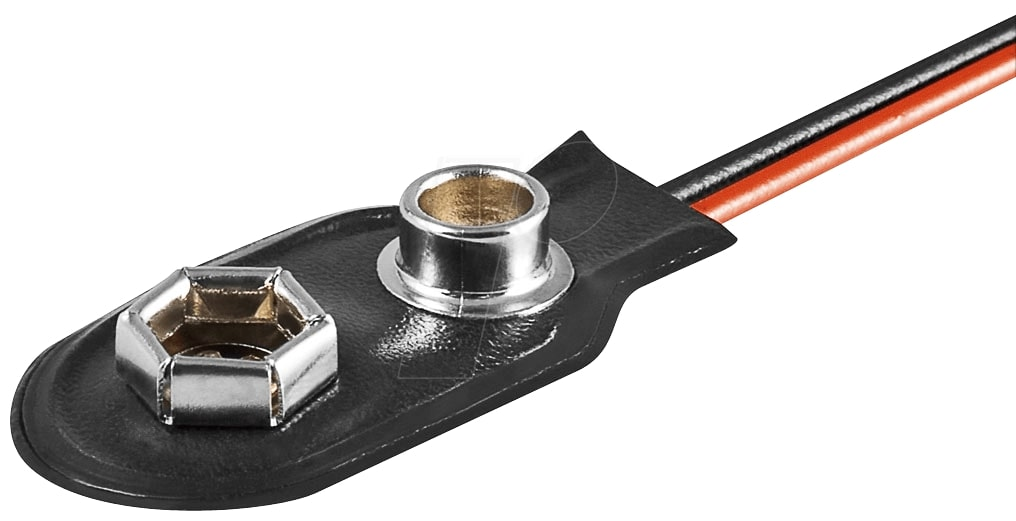
\includegraphics[width=3in]{Battery/clip.jpg}
        \caption{Batterieclip für 9-Volt-Block\cite{Reichelt:2024a}}
        \label{Batterieclip für 9-Volt-Block}
    \end{center}
\end{figure} 

\section{Spannungssensor}
Der Spannungssensor in Abb. \ref{Spannungssensor} von dem Hersteller \textit{Shenzhen Global Technology Co., Ltd} kann bei der Versorgungsspannung von 3,3 V Spannungen in dem Bereich von 0 V bis 16,5 V messen. Dieser wird genutzt, um den Ladestand der Batterie zu überwachen. Die analoge Auflösung des Sensors liegt bei 10 Bit. Damit kann bei dem angegebenen Messbereich die Spannung mit der Auflösung von 0,016 V gemessen werden. Zur Eingangsschnittstelle gehört der \ac{vcc}-Anschluss und der \ac{gnd}-Anschluss \cite{Shenzhen:2015}. Die Bauteilmaße betragen 13 mm x 27 mm.

\section{Spannungssensor}
Mit dem Sketch \FILE{TestBattery.ino} soll der Spannungssensor getestet werden.

\begin{code}[h]
    \pythonexternal[language=c++]{../../Code/Arduino/Battery/TestBattery.ino}
\end{code}

\subsection{Durchführung}

Für den Test werden die folgenden Hardware-Komponenten benötigt:

\begin{itemize}
    \item Arduino Nano 33 BLE Sense Lite
    \item Tiny Machine Learning Shield
    \item USB-A auf USB-Mikro Verbindungskabel
    \item Grove Jumper zu Grove 4 Pin Kabel
    \item Spannungssensor
    \item Batterie
    \item Batterieclip
\end{itemize}

Die Hardware-Komponenten werden  zusammengebaut, aber die Batterie wird noch nicht angeschlossen. Dann wird der Arduino Nano 33 BLE Sense Lite mit einem Computer verbunden. Anschließend wird der Sketch \FILE{TestBattery.ino} auf den Arduino Nano 33 BLE Sense Lite geladen und der serielle Monitor in der Arduino \acs{ide} geöffnet. Die Batterie wird während des Tests an den Batterieclip angeschlossen und der gemessene Wert bei dem seriellen Monitor ausgelesen.

\subsection{Ergebnisse}

Zu Beginn des Tests zeigt der serielle Monitor die Spannung 0 V an. Nach dem Anschließen der Batterie an den Spannungssensor wird die Spannung 9,6 V angezeigt.  Abbildung~\ref{BildSpannungTest} zeigt den gemessenen Spannungsverlauf. Die angezeigte Spannung liegt in dem erwarteten Bereich einer 9 V Batterie.

\begin{figure}[h]
    \begin{center}
        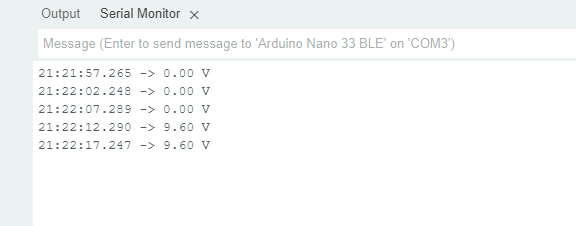
\includegraphics[width=\textwidth]{Battery/BatteryTest.png}
        \caption{Testoutput des Spannungssensors}
        \label{BildSpannungTest}
    \end{center}
\end{figure}

